\documentclass[12pt, twoside]{article}
\usepackage[letterpaper, margin=1in, headsep=0.5in]{geometry}
\usepackage[english]{babel}
\usepackage[utf8]{inputenc}
\usepackage{amsmath}
\usepackage{amsfonts}
\usepackage{amssymb}
\usepackage{tikz}
\usetikzlibrary{quotes, angles}
\usepackage{graphicx}
\usepackage{enumitem}
\usepackage{multicol}

\newif\ifmeta
\metatrue %print standards and topics tags

\title{Regents Geometry}
\author{Chris Huson}
\date{September 2020}

\usepackage{fancyhdr}
\pagestyle{fancy}
\fancyhf{}
\renewcommand{\headrulewidth}{0pt} % disable the underline of the header
\raggedbottom


\fancyhead[LE]{\thepage}
\fancyhead[RO]{\thepage \\ Name: \hspace{4cm} \,\\}
\fancyhead[LO]{BECA / Dr. Huson / Geometry}

\begin{document}

\subsubsection*{2.4 Exit Note: 7.G.B.5 Use angle facts; 8.EE.C.7.b Solve equations}
\begin{enumerate}
\item Identify the correct statement.
  \begin{multicols}{2}
    \begin{enumerate}
      \item $\angle 1 \cong \angle 4$
      \item $\angle 2 \cong \angle 3$
      \item $m\angle 1 + m\angle 2=90^\circ$
      \item $m\angle 1 + m\angle 2=180^\circ$
  \end{enumerate}
  \begin{center}
  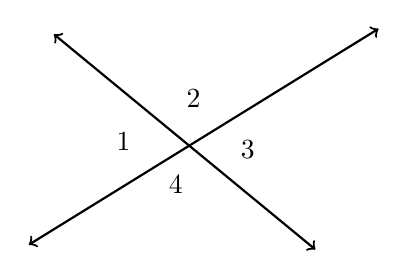
\begin{tikzpicture}[scale=0.5, rotate=15]
    \draw [<->, thick] (0,-1.5)--(10,1.5);
    \draw [<->, thick] (2,3.5)--(7,-3.5);
    \node at (3,.4){1};
    \node at (6,-.6){3};
    \node at (5,1){2};
    \node at (4,-1){4};
  \end{tikzpicture}
  \end{center}
\end{multicols} 
Given that $m\angle 1=3x-10$, $m\angle 2=2x+40$, $m\angle 3=2x+20$, and $m\angle 4=4x-20$. Use the equation you chose in the first part to find $x$.
\vspace{6cm}

\item The ray $\overrightarrow{BD}$ bisects $\angle ABC$. Given $m\angle ABD = 3x+7$ and \\$m\angle DBC = 4x-9$. Identify the true statement(s).
 \begin{multicols}{2}
    \begin{enumerate}
      \item $\angle ABD$, $\angle DBC$ are adjacent and\\
      $4x-9 =180^\circ$
      \item $\angle ABD$ and $\angle DBC$ are a linear pair\\
      $(3x+7) + (4x-9)=180^\circ$
      \item $\angle ABD \cong \angle DBC$\\
      $3x+7 = 4x-9$
  \end{enumerate}
  \begin{center}
    \begin{tikzpicture}[scale=0.6, rotate=0]
      \draw [<->, thick] (130:5)node[below left]{$A$} 
      --(0,0)node[below left]{$B$}
      --(20:5)node[above right]{$C$};
      \draw [->, thick] (0,0)--(75:5)node[left]{$D$};
    \end{tikzpicture}
  \end{center}
\end{multicols}
Copy the correct equation and find $m\angle ABD$. Check your answer. 

\newpage
\item Identify the true statement(s) given $\angle AOB = 4x-4$ and $\angle DOE = 6x-26$.
  \begin{multicols}{2}
     \begin{enumerate}
       \item $\angle AOB$, $\angle DOE$ are complementary\\
       $(4x-4) + (6x-26)=90^\circ$
       \item $\angle AOB \cong \angle DOE$ are vertical angles,\\
       $4x-4 = 6x-26$
       \item $\angle AOB$ and $\angle DOE$ are a linear pair\\
       $(4x-4) + (6x-26)=180^\circ$
   \end{enumerate}
   \begin{center}
     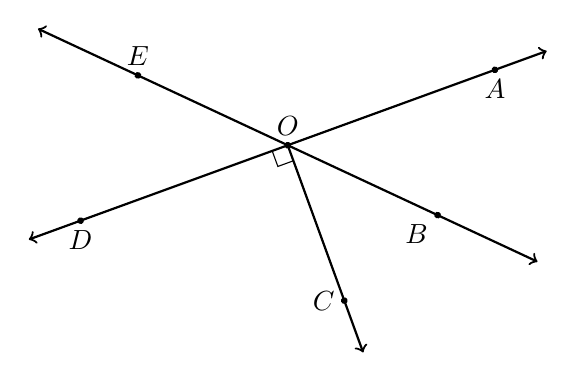
\begin{tikzpicture}[scale=0.7, rotate=200]
       \draw [<->, thick] (-45:5)--(0,0)--(135:5);
       \draw [<->, thick] (-5,0)--(5,0);
       \draw [->, thick] (0,0)--(0,4);
       \draw (0,0)++(0.3,0)--++(0,0.3)--+(-0.3,0);
       \draw [fill] (135:3) circle [radius=0.05] node[below left]{$B$};
       \draw [fill] (-4,0) circle [radius=0.05] node[below]{$A$}; 
       \draw [fill] (0,0) circle [radius=0.05] node[above]{$O$};
       \draw [fill] (0,3) circle [radius=0.05] node[left]{$C$};
       \draw [fill] (4,0) circle [radius=0.05] node[below]{$D$};
       \draw [fill] (-45:3) circle [radius=0.05] node[above]{$E$};
       \end{tikzpicture}
   \end{center}
 \end{multicols}
 Copy the correct equation and solve for $x$. Check your answer. \vspace{6cm}

\item The ray $\overrightarrow{KM}$ bisects $\angle JKL$. Given $m\angle JKM = 5x+k$ and \\$m\angle JKL = 12x-34+2k$.
 \begin{multicols}{2}
    \begin{enumerate}
      \item Find $x$.
      \item Given that $\angle JKM$ is obtuse, what are the potential values of $k$?
  \end{enumerate} \vspace{2cm}
  \begin{center}
    \begin{tikzpicture}[scale=0.6, rotate=-10]
      \draw [<->, thick] (190:5)node[below left]{$J$} 
      --(0,0)node[below left]{$K$}
      --(0:5)node[above right]{$L$};
      \draw [->, thick] (0,0)--(95:5)node[below left]{$M$};
      %\draw [fill] (0,0) circle [radius=0.05] node[below]{$A$};
      %\draw [fill] (5,0) circle [radius=0.05] node[below]{$B$};
    \end{tikzpicture}
  \end{center}
\end{multicols}

\end{enumerate}
\end{document}